\begin{frame}
\frametitle{Corps humain / Résultats}
\vfill
\begin{columns}
\column{0.6\textwidth}
%\scalebox{0.9}{\begin{minipage}{1.11\textwidth}
\begin{figure}
\begin{tabular}{|l|c|c|}
	\hline
	Critère & GD1-RK2 & GD2-RK2 \\ \hline\hline
	Nombre de mailles & 23.4 M & 23.4 M \\	\hline
	Nombre d'inconnues & 1123 M & 3791 M \\	\hline
	Mémoire & 40 Go & 100 Go \\	\hline
\end{tabular}
\end{figure}
\vfill
\begin{itemize}
\item Temps physique simulé : 10 ns ;
\item Machine AxesSim :\\ 8 GPU NVidia GeForce GTX 1080 Ti 11 Go ;
\item Temps machine GD1-RK2 : 2072 heures ;
\item Temps humain GD1-RK2 : 10.79 jours.
\end{itemize}
%\end{minipage}}
\vfill
\begin{figure}
\centering
\href{run:../img/modE_xoz_ogv.mp4}{\textcolor{blue}{VIDEO plan (xOz)}}

1 s de vidéo $\leftrightarrow$ 6.5 h de calcul intensif

1 s de vidéo $\leftrightarrow$ 0.25 ns physiques
\end{figure}
\column{0.4\textwidth}
\begin{figure}
\centering
(xOz), $t = 3$ ns.

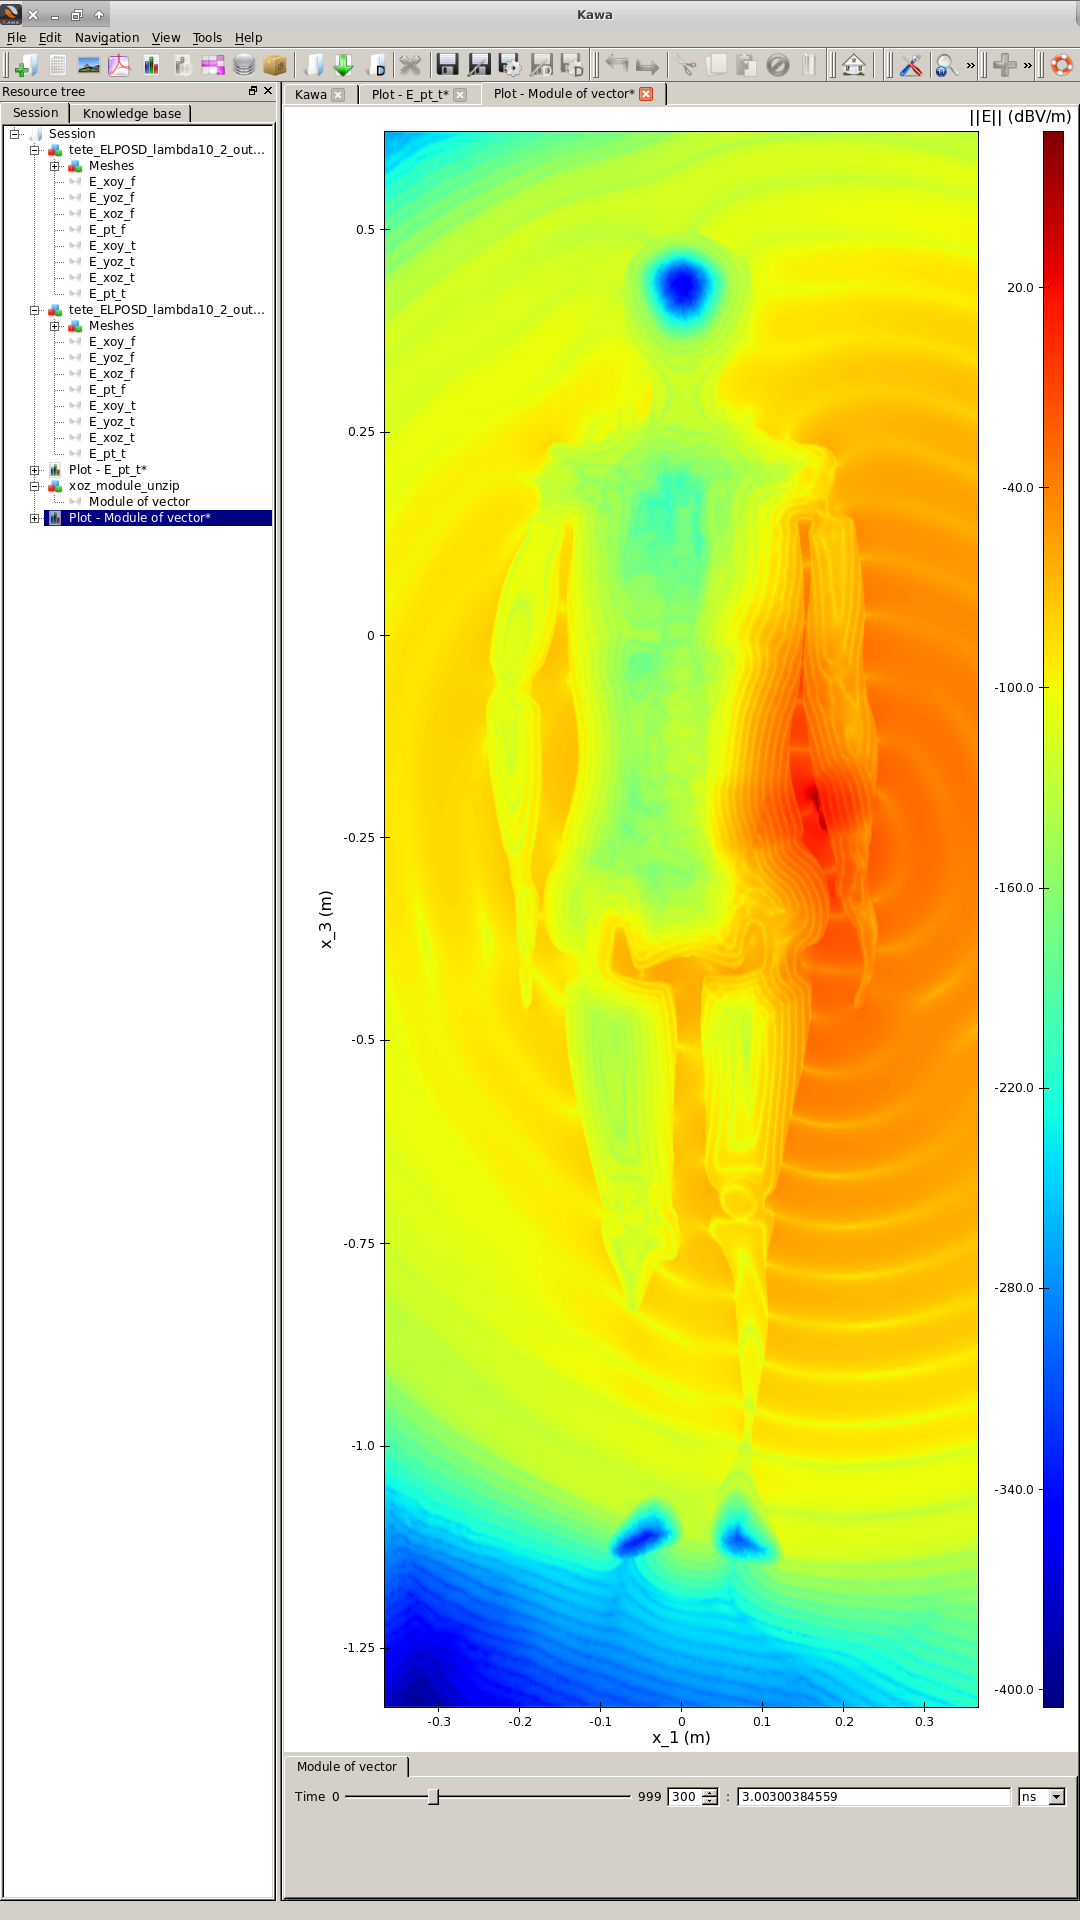
\includegraphics[
	width=0.66\linewidth,
	trim={317 170 8 108},clip
	]{../img/kyoto_3ns}
\end{figure}
\end{columns}
\vfill
\end{frame}

